\documentclass[conference]{IEEEtran}
\IEEEoverridecommandlockouts
% The preceding line is only needed to identify funding in the first footnote. If that is unneeded, please comment it out.
%Template version as of 6/27/2024

\usepackage{cite}
\usepackage{amsmath,amssymb,amsfonts}
\usepackage{algorithmic}
\usepackage{graphicx}
\usepackage{textcomp}
\usepackage{xcolor} 
\usepackage{hyperref}
\usepackage{cleveref}
\def\BibTeX{{\rm B\kern-.05em{\sc i\kern-.025em b}\kern-.08em
    T\kern-.1667em\lower.7ex\hbox{E}\kern-.125emX}}
\usepackage{siunitx}

% By Pascal
\let\bm\mathbf
\usepackage{tabularx,booktabs}
\usepackage{url}
\usepackage{subcaption}
\usepackage{pgfmath}
\usepackage{float}
\usepackage{comment}
\usepackage{enumitem}
\usepackage{multirow}
\sisetup{detect-all=true}

\newcommand\formatpercentage[2][round-precision = 1]{%
    \SI[round-mode = places,
        scientific-notation = fixed, fixed-exponent = 0,
        output-decimal-marker={.}, #1]{#2e2}{\percent}%
}

\newcommand\formatpercentagebold[2][round-precision = 1]{%
    \textbf{\SI[round-mode = places,
        scientific-notation = fixed, fixed-exponent = 0,
        output-decimal-marker={.}, #1]{#2e2}{\percent}}%
}

\crefname{figure}{Fig.}{Figures}
\Crefname{figure}{Fig.}{Figures}
\crefname{section}{Section}{Sections}
\Crefname{section}{Section}{Sections}
\crefname{equation}{Eq.}{Eqs.}
\Crefname{equation}{Eq.}{Eqs.}
\crefname{appendix}{Appendix}{Appendix}
\Crefname{appendix}{Appendix}{Appendix}
\crefname{table}{Table}{Table}
\Crefname{table}{Table}{Table}

\begin{document}

\title{Hounsfield Unit Ranges as Inductive Bias for Intra-Clinical Learning of Data-Efficient\\CT Segmentation Models\\
\thanks{This work has been supported by the research council of the Cantonal Hospital of Aarau grant FR1410.000.156.}
}
\author{
    %Block for anonymous Submission
    %\IEEEauthorblockN{anonymous authors}
    %\IEEEauthorblockA{email}
    %\IEEEauthorblockA{affiliation}
    %\IEEEauthorblockA{}
    %\IEEEauthorblockA{}
    %\IEEEauthorblockA{}
    \IEEEauthorblockN{\href{https://orcid.org/0009-0006-5609-2700}{
\includegraphics[scale=0.08]{figures/orcid.pdf}}\hspace{1mm}Benjamin Meyer\IEEEauthorrefmark{1}\IEEEauthorrefmark{2}\IEEEauthorrefmark{6}, 
    \href{https://orcid.org/0000-0002-8084-2317}{
\includegraphics[scale=0.08]{figures/orcid.pdf}}\hspace{1mm}Pascal J. Sager\IEEEauthorrefmark{1}\IEEEauthorrefmark{2}\IEEEauthorrefmark{6},\\
    \href{https://orcid.org/0000-0003-4679-8081}{
\includegraphics[scale=0.08]{figures/orcid.pdf}}\hspace{1mm}Ahmed Abdulkadir\IEEEauthorrefmark{1},
    \href{https://orcid.org/0000-0001-8560-2120}{
\includegraphics[scale=0.08]{figures/orcid.pdf}}\hspace{1mm}Benjamin F. Grewe\IEEEauthorrefmark{2},
    \href{https://orcid.org/0000-0001-6400-4949}{
\includegraphics[scale=0.08]{figures/orcid.pdf}}\hspace{1mm}Philipp Schuetz\IEEEauthorrefmark{3}, 
    \href{https://orcid.org/0000-0002-3784-0420}{
\includegraphics[scale=0.08]{figures/orcid.pdf}}\hspace{1mm}Thilo Stadelmann\IEEEauthorrefmark{1}\IEEEauthorrefmark{5},
    \href{https://orcid.org/0000-0002-4362-162X}{
\includegraphics[scale=0.08]{figures/orcid.pdf}}\hspace{1mm}Felice Burn\IEEEauthorrefmark{4}}
    % \IEEEauthorblockA{\{mebr,sage,stdm\}@zhaw.ch, bgrewe@ethz.ch, \{philipp.schuetz,felice.burn\}@ksa.ch}
    \IEEEauthorblockA{\{mebr,sage,abdk,stdm\}@zhaw.ch, bgrewe@ethz.ch, \{philipp.schuetz,felice.burn\}@ksa.ch}
    \IEEEauthorblockA{\IEEEauthorrefmark{1}Centre for Artificial Intelligence, Zurich University of Applied Sciences, Winterthur, Switzerland}
    \IEEEauthorblockA{\IEEEauthorrefmark{2}Institute of Neuroinformatics, ETH Zurich \& University of Zurich, Zurich, Switzerland}
    \IEEEauthorblockA{\IEEEauthorrefmark{3}University Clinic of Medicine, Aarau Cantonal Hospital, Aarau, Switzerland}
    \IEEEauthorblockA{\IEEEauthorrefmark{4}AI \& Data Science CoE, Aarau Cantonal Hospital, Aarau, Switzerland}
    \IEEEauthorblockA{\IEEEauthorrefmark{5}Fellow, ECLT (European Centre for Living Technology, Venice, Italy) and Senior Member, IEEE}
    \IEEEauthorblockA{\IEEEauthorrefmark{6}The first two authors contributed equally to this work.}
}

\author{
    %Block for anonymous Submission
    %\IEEEauthorblockN{anonymous authors}
    %\IEEEauthorblockA{email}
    %\IEEEauthorblockA{affiliation}
    %\IEEEauthorblockA{}
    %\IEEEauthorblockA{}
    %\IEEEauthorblockA{}
    \IEEEauthorblockN{\href{https://orcid.org/0009-0006-5609-2700}{
\includegraphics[scale=0.08]{figures/orcid.pdf}}\hspace{1mm}Benjamin Meyer\IEEEauthorrefmark{1}\IEEEauthorrefmark{2}\IEEEauthorrefmark{6}, 
    \href{https://orcid.org/0000-0002-8084-2317}{
\includegraphics[scale=0.08]{figures/orcid.pdf}}\hspace{1mm}Pascal J. Sager\IEEEauthorrefmark{1}\IEEEauthorrefmark{2}\IEEEauthorrefmark{6},\\
    \href{https://orcid.org/0000-0003-4679-8081}{
\includegraphics[scale=0.08]{figures/orcid.pdf}}\hspace{1mm}Ahmed Abdulkadir\IEEEauthorrefmark{1},
    \href{https://orcid.org/0000-0001-8560-2120}{
\includegraphics[scale=0.08]{figures/orcid.pdf}}\hspace{1mm}Benjamin F. Grewe\IEEEauthorrefmark{2},
    \href{https://orcid.org/0000-0001-6400-4949}{
\includegraphics[scale=0.08]{figures/orcid.pdf}}\hspace{1mm}Philipp Schuetz\IEEEauthorrefmark{3}, 
    \href{https://orcid.org/0000-0002-3784-0420}{
\includegraphics[scale=0.08]{figures/orcid.pdf}}\hspace{1mm}Thilo Stadelmann\IEEEauthorrefmark{1}\IEEEauthorrefmark{5},
    \href{https://orcid.org/0000-0002-4362-162X}{
\includegraphics[scale=0.08]{figures/orcid.pdf}}\hspace{1mm}Felice Burn\IEEEauthorrefmark{4}}
    % \IEEEauthorblockA{\{mebr,sage,stdm\}@zhaw.ch, bgrewe@ethz.ch, \{philipp.schuetz,felice.burn\}@ksa.ch}
    \IEEEauthorblockA{\{mebr,sage,abdk,stdm\}@zhaw.ch, bgrewe@ethz.ch, \{philipp.schuetz,felice.burn\}@ksa.ch}
    \IEEEauthorblockA{\IEEEauthorrefmark{1}Centre for Artificial Intelligence, Zurich University of Applied Sciences, Winterthur, Switzerland}
    \IEEEauthorblockA{\IEEEauthorrefmark{2}Institute of Neuroinformatics, ETH Zurich \& University of Zurich, Zurich, Switzerland}
    \IEEEauthorblockA{\IEEEauthorrefmark{3}University Clinic of Medicine, Aarau Cantonal Hospital, Aarau, Switzerland}
    \IEEEauthorblockA{\IEEEauthorrefmark{4}AI \& Data Science CoE, Aarau Cantonal Hospital, Aarau, Switzerland}
    \IEEEauthorblockA{\IEEEauthorrefmark{5}Fellow, ECLT (European Centre for Living Technology, Venice, Italy) and Senior Member, IEEE}
    \IEEEauthorblockA{\IEEEauthorrefmark{6}The first two authors contributed equally to this work.}
}

\maketitle

\begin{abstract}
Automated tissue segmentation in medical imaging plays a critical role in clinical AI-assisted decision-making, and particularly in the assessment of body composition from CT scans.
However, acquiring data and annotations of sufficient quality to train deep-learning models is expensive and time-consuming.
In this work, we propose a novel approach to improve data efficiency and model accuracy by leveraging domain knowledge about biologically relevant tissue-specific Hounsfield unit (HU) ranges as an inductive bias for learning. 
Specifically, we extend the input representation of deep learning-based segmentation models with binary masks indicating potential tissue types, where each binary mask is created from thresholds derived from medical literature.
Our method not only enhances segmentation performance by up to \SI{5}{\percent} for intramuscular adipose tissue but surpasses the performance of the baseline model
with \SI{50}{\percent} of the training data.
Our easy-to-apply method thus improves data efficiency and facilitates the development and use of segmentation models in resource-constrained clinical settings.
\end{abstract}

\begin{IEEEkeywords}
Tissue segmentation, body composition analysis, medical imaging, data efficiency, physiology-informed machine learning, deep learning
\end{IEEEkeywords}

\section{Introduction}
%
%
%
% Introduction into the problem
Deep neural networks have shown remarkable performance across various domains, including health and medical imaging \cite{schmidhuber2015deep, stadelmann2019beyond, emberger2023video, amirian2023mitigation}.
They have huge potential in clinical decision support systems, assisting physicians in making more informed diagnoses and better treatment choices \cite{kose_deep_2021, kabir_deep_2023, jermain2024deep}.
An important task in medical imaging is the assessment of a patient’s body composition \cite{ali_sarcopenia_2014}, such as quantifying muscle mass and different types of adipose tissue \cite{tolonen_methodology_2021}.
A widely adopted approach for estimating body composition is applying tissue segmentation to a specific two-dimensional (2D) slice extracted from a three-dimensional computed tomography (CT) scan.
Tissue segmentation labels the tissue type at the pixel level, allowing for the calculation of tissue areas and subsequent body composition analysis (BCA).
% The 2D slice for segmentation is typically taken at the level of the first (L1)  \cite{tolonen_methodology_2021} or third lumbar vertebra (L3) \cite{amini_approaches_2019} as well as the tenth (T10) \cite{derstine2018skeletal} or twelfth thoracic vertebra (T12) \cite{tolonen_methodology_2021}.

\begin{figure}[t]
\centering
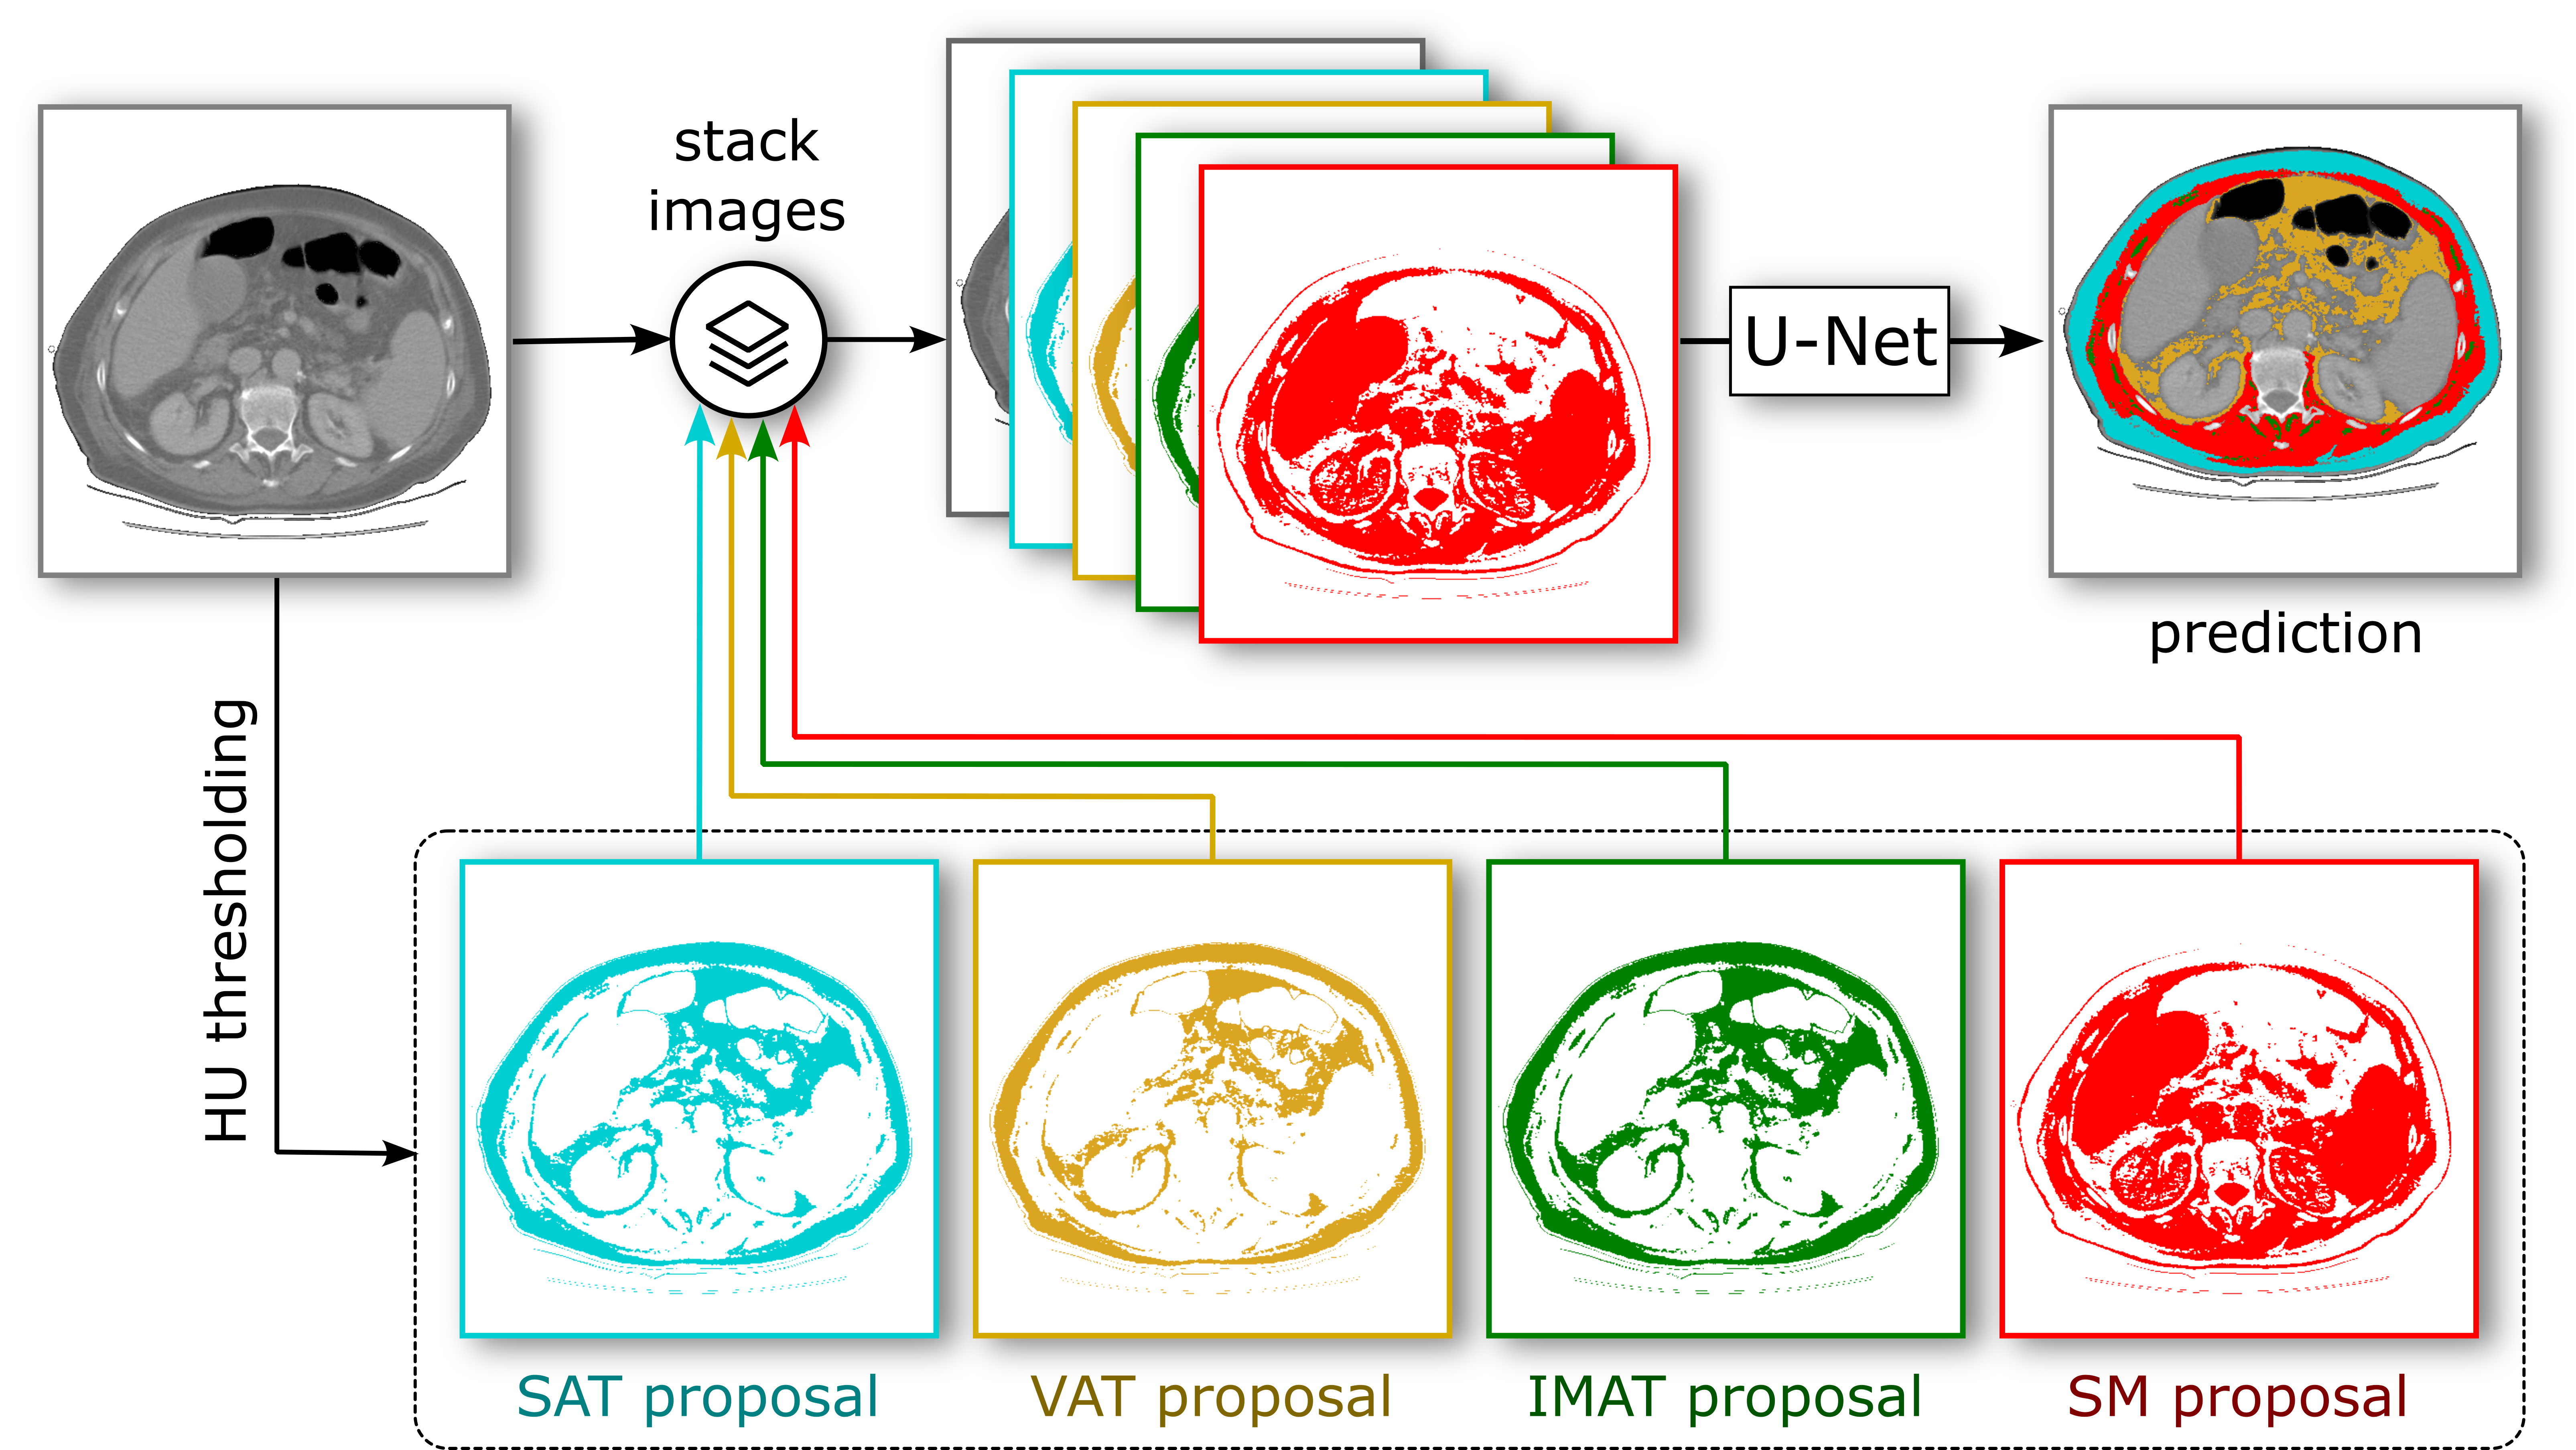
\includegraphics[width=0.5\textwidth]{figures/overview3.png}
\caption{Overview of our approach: Binary masks that indicate potential tissue-specific locations are extracted using HU ranges as thresholds and concatenated with the original CT image as additional input channels for a machine learning model.}
\label{fig:overview}
\end{figure}

% What is the problem
Despite the importance of automated BCA, only a few publicly ready-to-use systems with limited scope exist \cite{wasserthal2023totalsegmentator,makrakis2023effect,dietz2025evaluation}. 
Furthermore, annotated datasets are rarely shared due to strong data privacy constraints and strict regulations regarding medical data usage.
Consequently, institutions such as hospitals and software manufacturers must train (or fine-tune) custom segmentation models on internal annotated data to adapt to in-house imaging equipment and procedures \cite{amirian2021prepnet, sager_unsupervised_2022}.
The necessary annotations must be provided by medical experts, such as radiologists, making the labeling process both expensive and time-intensive to the point of infeasibility given ordinary clinical operations as a main task. 
This raises our research question:
\emph{How can the number of required training samples be reduced for machine learning-based medical imaging models while maintaining the performance necessary for clinical application?}

% What others do
Existing approaches to mitigate data scarcity in medical segmentation use techniques like data augmentation, transfer learning, domain adaptation, or self-supervised techniques (for a detailed review, see Section \ref{sec:related-work-labels}).
While these techniques can reduce the dependency on annotated data, they often require careful optimization of hyperparameters, model architectures, and learning strategies, making them complex to implement effectively.

%What we do
In this paper, we introduce an easy-to-apply approach to reduce the dependence on labeled training data.
Specifically, taking the data-centric perspective \cite{stadelmann2022data, luley2023concept} into account, we leverage established tissue-specific ranges of so-called Hounsfield unit (HU) values from the medical literature, defined on the Hounsfield scale (a standardized measure of radiodensity in CT imaging), as an inductive bias to learn segmentation models:
Each tissue type exhibits a well-defined HU range \cite{beaudart_sarcopenia_2016}, providing natural prior knowledge that can guide the learning process.
For instance, cortical bone typically falls within the range of $+500$ to $+1900$ HU, whereas different adipose tissue is found within $-190$ to $-30$ HU \cite{mueller2023association}.
By incorporating HU ranges as prior knowledge, the model is informed about plausible tissue types for each pixel and can use this information as an inductive bias to guide learning, thereby narrowing the search space and improving data efficiency as well as segmentation performance.
%

% Contributions
We make the following contributions: (1) \emph{Utilization of HU ranges:} We propose incorporating HU ranges as a novel and effective inductive bias to learn tissue segmentation economically and enhance the final neural network's performance. (2) \emph{Comprehensive experiments:} We conduct extensive experiments across various model and dataset sizes, demonstrating robust improvements. (3) \emph{Tissue-level analysis:} We highlight that our method is especially helpful for identifying intra-muscular adipose tissue (IMAT), a clinically relevant tissue type representing muscle health conditions.
Our contributions have direct relevance for clinical practice, enabling the efficient training and clinical application of tailored segmentation models in-house.

\section{Related Work} \label{sec:related-work}

\subsection{Abdominal CT segmentation for BCA}
CT, alongside magnetic resonance imaging (MRI), is considered the most accurate modality for BCA \cite{beaudart_sarcopenia_2016}, where different tissue types are classified at the pixel level.
It has been demonstrated that 2D slices acquired at the level of the first (L1)  \cite{tolonen_methodology_2021} or third lumbar vertebra (L3) \cite{amini_approaches_2019} as well as the tenth (T10) \cite{derstine2018skeletal} or twelfth thoracic vertebra (T12) \cite{cho2019association} serve as a reliable surrogate by segmenting for the assessment of abdominal body compositions, enabling an efficient estimation of body composition without requiring full-volume segmentation \cite{shen_total_2004}.
For a comprehensive discussion on alternative anatomical levels, refer to \cite{tolonen_methodology_2021}.
Recent advancements in automated BCA predominantly utilize deep learning-based segmentation models, particularly U-Net architectures \cite{paris_automated_2020, hemke_deep_2020, koitka_fully_2021} or variations of it \cite{dabiri_muscle_2019}.
These models are trained on CT slices where each pixel's value corresponds to a Hounsfield Unit (HU), enabling the model to learn the relationship between HU values and tissue types.

In this study, we build upon these existing methodologies and enhance the well-established U-Net framework \cite{navab_u-net_2015} by incorporating \emph{HU ranges}, derived from the medical literature as an inductive bias during pre-processing. By leveraging medical textbook knowledge in this manner, we employ an effective inductive bias that facilitates more data-efficient learning and enhances final segmentation performance.

\subsection{Label scarcity in medical image segmentation} \label{sec:related-work-labels}
Various methodologies have been developed to address the challenge of missing or partially labeled segmentation data \cite{simmler_survey_2021}.
\emph{Data augmentation} techniques artificially expand the dataset by applying transformations to the original data, thereby generating multiple variations \cite{gardner_realistic_2023, goceri_medical_2023, tuggener_real_2024, lim2025transraunet}.
\emph{Domain adaptation and transfer learning} facilitate knowledge transfer from related domains or tasks, enhancing model generalization \cite{amirian2021prepnet, guan_domain_2022, karimi_transfer_2021, yan2024comprehensive}.
\emph{Weakly-supervised learning} leverages unlabeled data in conjunction with limited annotations to improve model performance \cite{sager_unsupervised_2022, felfeliyan_self-supervised-rcnn_2023}.

Similar to data augmentation, we use a pre-processing step (creation of HU range-based binary masks) that is applied before model training. 
However, rather than expanding the dataset by new examples, our method enriches each example with additional domain knowledge  (fed into the network as additional channels of the original input example), akin to approaches in other domains such as physics-informed neural networks \cite{cuomo_scientific_2022}. This creates strong physiology-informed inductive biases in neural network training.

Prior research has demonstrated that incorporating domain knowledge into medical imaging is a highly effective strategy for addressing label scarcity \cite{sager_unsupervised_2022}.
For example, a related approach is \emph{HU window} pre-processing \cite{kloenne_domain-specific_2020,steybe2022automated} that normalizes and clips HU values rather than deriving simple binary masks (for details, see \cref{sec:hu-windowing}).
Importantly, our approach is complementary to existing methodologies, offering a versatile addition to current techniques for reducing data requirements in medical segmentation.


\section{Hounsfield Unit Ranges as Inductive Bias}
The goal of tissue segmentation for BCA is to classify each pixel of a 2D CT slice into a tissue class or the background class.
We denote the CT slice, a 2D image of HU values, as matrix $\bm{X}_0 \in \mathbb{R}^{h, w}$, where $h$ and $w$ denote the height and width of the slice.
The HU pixel values in $\bm{X}_0$ typically range from $-\num{1000}$ (air) to approximately $+\num{3000}$ (dense bone) \cite{bibb2014medical}, while foreign objects such as metal implants can exhibit HU values up to $+\num{30000}$.
The pixel-wise classification outputs a segmentation mask $\hat{\bm{Y}} \in (\mathcal{C} \cup \{ BG \})^{h , w}$ of the same shape as the input image, where $\mathcal{C}$ represents the set of tissue classes and $BG$ the background class.

\Cref{fig:overview} visualizes how we integrate the prior knowledge about tissue-specific HU ranges into the model.
On top of the input $\bm{X}_0$ we stack $|\mathcal{C}|$ binary masks $\{ \bm{X}_c\ |\ c \in \mathcal{C}\}$, yielding $\bm{X} \in \mathbb{R}^{(1 + |\mathcal{C}|) , h , w}$. 
Given $\bm{X}_0(i,j)$ be the pixel value at row $i$ and column $j$ in matrix $\bm{X}_0$, $\bm{X}_c$ for class $c$ is defined as:
% 
\begin{equation*}
\bm{X}_{c}(i,j)=\begin{cases}
    1, & \text{if } \bm{X}_{0}(i,j) \text{ within the HU range of class } c,\\
    0, & \text{otherwise}.
\end{cases}
\label{eq:pixel_indicator}
\end{equation*}

Thus, the first channel of the input $\bm{X}$ contains the ``original'' CT image $\bm{X}_0$, while the additional channels contain the binary masks $\bm{X}_c$, each indicating if a class $c$ is plausible at specific pixel locations according to medical textbook knowledge on HU ranges.
%
\begin{table}[t]
    \caption{HU ranges for each tissue type.}
    \begin{center}
        \begin{tabular}{lcc}
        \toprule
        \textbf{Tissue type} & \multicolumn{2}{c}{\textbf{HU range}} \\
        \cmidrule(lr){2-3}
         & \textbf{From} & \textbf{To} \\
        \midrule
        Skeletal muscle (SM) & -29 & 150 \\
        Intramuscular adipose tissue (IMAT) & -190 & -30 \\
        Visceral adipose tissue (VAT) & -150 & -50 \\
        Subcutaneous adipose tissue (SAT) & -190 & -30 \\
        \bottomrule
        \end{tabular}
    \label{tab:hu_values}
    \end{center}
\end{table}
%
\Cref{tab:hu_values} provides an overview of the tissue types and corresponding HU ranges used in this study. 
Equivalent HU ranges (IMAT, SAT) lead to identical binary masks and could also be represented as a single mask.
Overlapping HU ranges (e.g., VAT, SAT) lead to overlapping masks, indicating multiple possible tissue types at some locations.
Adding the respective information as additional input channels effectively constrains the model’s decision space, reducing ambiguity and improving segmentation accuracy by leveraging well-established radiodensity properties.


\section{Experimental Setup}

We evaluate our proposed approach using widely adopted deep learning architectures for medical image segmentation, training them with default hyperparameter settings. To ensure a rigorous assessment, we employ standard validation procedures in accordance with best practices.

\subsection{Model}
For the segmentation task, we build upon a 2D U-Net model~\cite{navab_u-net_2015}, a widely recognized state-of-the-art architecture in this domain, known for its effectiveness even in data-limited scenarios. The U-Net model follows an encoder-decoder structure with skip connections to preserve spatial information. To test our approach on different model sizes, we train three model variants with different initial feature map sizes ($16$, $32$, or $64$ channels). All configurations are based on a standard U-Net architecture and maintain a consistent depth of five encoding and decoding stages. They follow the standard practice of doubling the number of feature maps at each downsampling stage and ending with a $1\times1$ kernel for pixel-wise prediction \cite{navab_u-net_2015}. The models contain around 2M (\emph{U-Net-small}), 8M (\emph{U-Net-base}), and 31M (\emph{U-Net-large}) parameters, respectively.

Unlike the original U-Net architecture, we employ padded convolutions and add batch normalization after each convolutional layer in the encoder and decoder.
% No dropout or other regularization was employed.

\subsection{Data}
We conduct our experiments using CT data obtained from the Cantonal Hospital Aarau, Switzerland. 
Our dataset contains $176$ CT slices in $512 \times 512$ resolution from $44$ patients with malnutritional conditions.
We segment four tissue types: The skeletal muscle (SM), intramuscular adipose tissue (IMAT), visceral adipose tissue (VAT), and subcutaneous adipose tissue (SAT).
For each patient, we label four CT slices acquired at the vertebral levels: L1, L3, T10, and T12.
All patients gave general consent for research purposes, although due to data privacy regulations and national legislation (HRA), we are unable to publicly share imaging data, associated annotations, or model predictions.

To demonstrate the effectiveness of our approach on different dataset sizes, we sample subsets only containing fractions (\SI{10}{\percent}, \SI{20}{\percent}, $\dots$, \SI{100}{\percent}) of the available data.
The subsets are \emph{nested}, meaning a bigger subset includes smaller subsets, simulating the growth of an increasingly large dataset.

\subsection{Annotation process}
Following a thorough review, one case was removed due to unsuitable quality for manual analysis, as skeletal muscle tissue extended beyond the field of view. No further exclusion was needed due to, e.g., severe anatomical or technical abnormalities, such as body habitus variations, metal artifacts, or massive fluid accumulation. The remaining slices were classified based on characteristics commonly encountered in routine CT scans, including subcutaneous adipose tissue extending beyond the image field and mild image quality impairments (e.g., streaking or graininess). After dataset review, all eligible slices underwent semi-assisted manual segmentation using Slicomatic™ software from TomoVision at the specified vertebral levels \cite{baumgartner2023association}.

\subsection{Training parameters}
% No dedicated hyperparameter tuning was performed to isolate the impact of our feature engineering.
Each model is trained using the standard Adam optimizer~\cite{kingma2014adam} with its default settings: learning rate $\alpha=0.001$, $\beta_1=0.9$, $\beta_2=0.999$, and $\epsilon=10^{-8}$. The optimization process minimizes the cross-entropy loss function using a batch size of $4$.
Regardless of the dataset fraction used, we maintain a fixed number of \num{1800} optimization steps across all settings to ensure convergence and fair comparison of model performance.

\subsection{Validation}
All experiments are conducted using a 3-fold cross-validation across patients.
Folds are generated using the same random seed, enabling consistent comparisons across all experiments.

Performance metrics are reported as the mean value computed across the three folds. For each fold, all evaluation metrics are computed based on the best model checkpoint, as determined by the lowest validation loss.
We report the Dice score, which quantifies the overlap between the predicted segmentation ($P$) and the ground truth segmentation ($G$) and is defined as:
%
\begin{equation*}
\frac{2 \cdot |P \cap G|}{|P| + |G|}
\end{equation*}
%
Additionally, we report the precision, the recall, and the F$_1$ score.
All metrics are macro-averaged (calculated per tissue class and then averaged across classes), which is common practice to account for class imbalance.
To quantify the uncertainty in the estimated means, we report the \SI{95}{\percent} confidence interval, estimated using the standard deviation across folds. % Additionally, for each fold, all evaluation metrics are computed based on the best model checkpoint, as determined by the lowest validation loss.



\section{Results}

\subsection{Reduced data needs}

\begin{figure}[t]
    \centering
    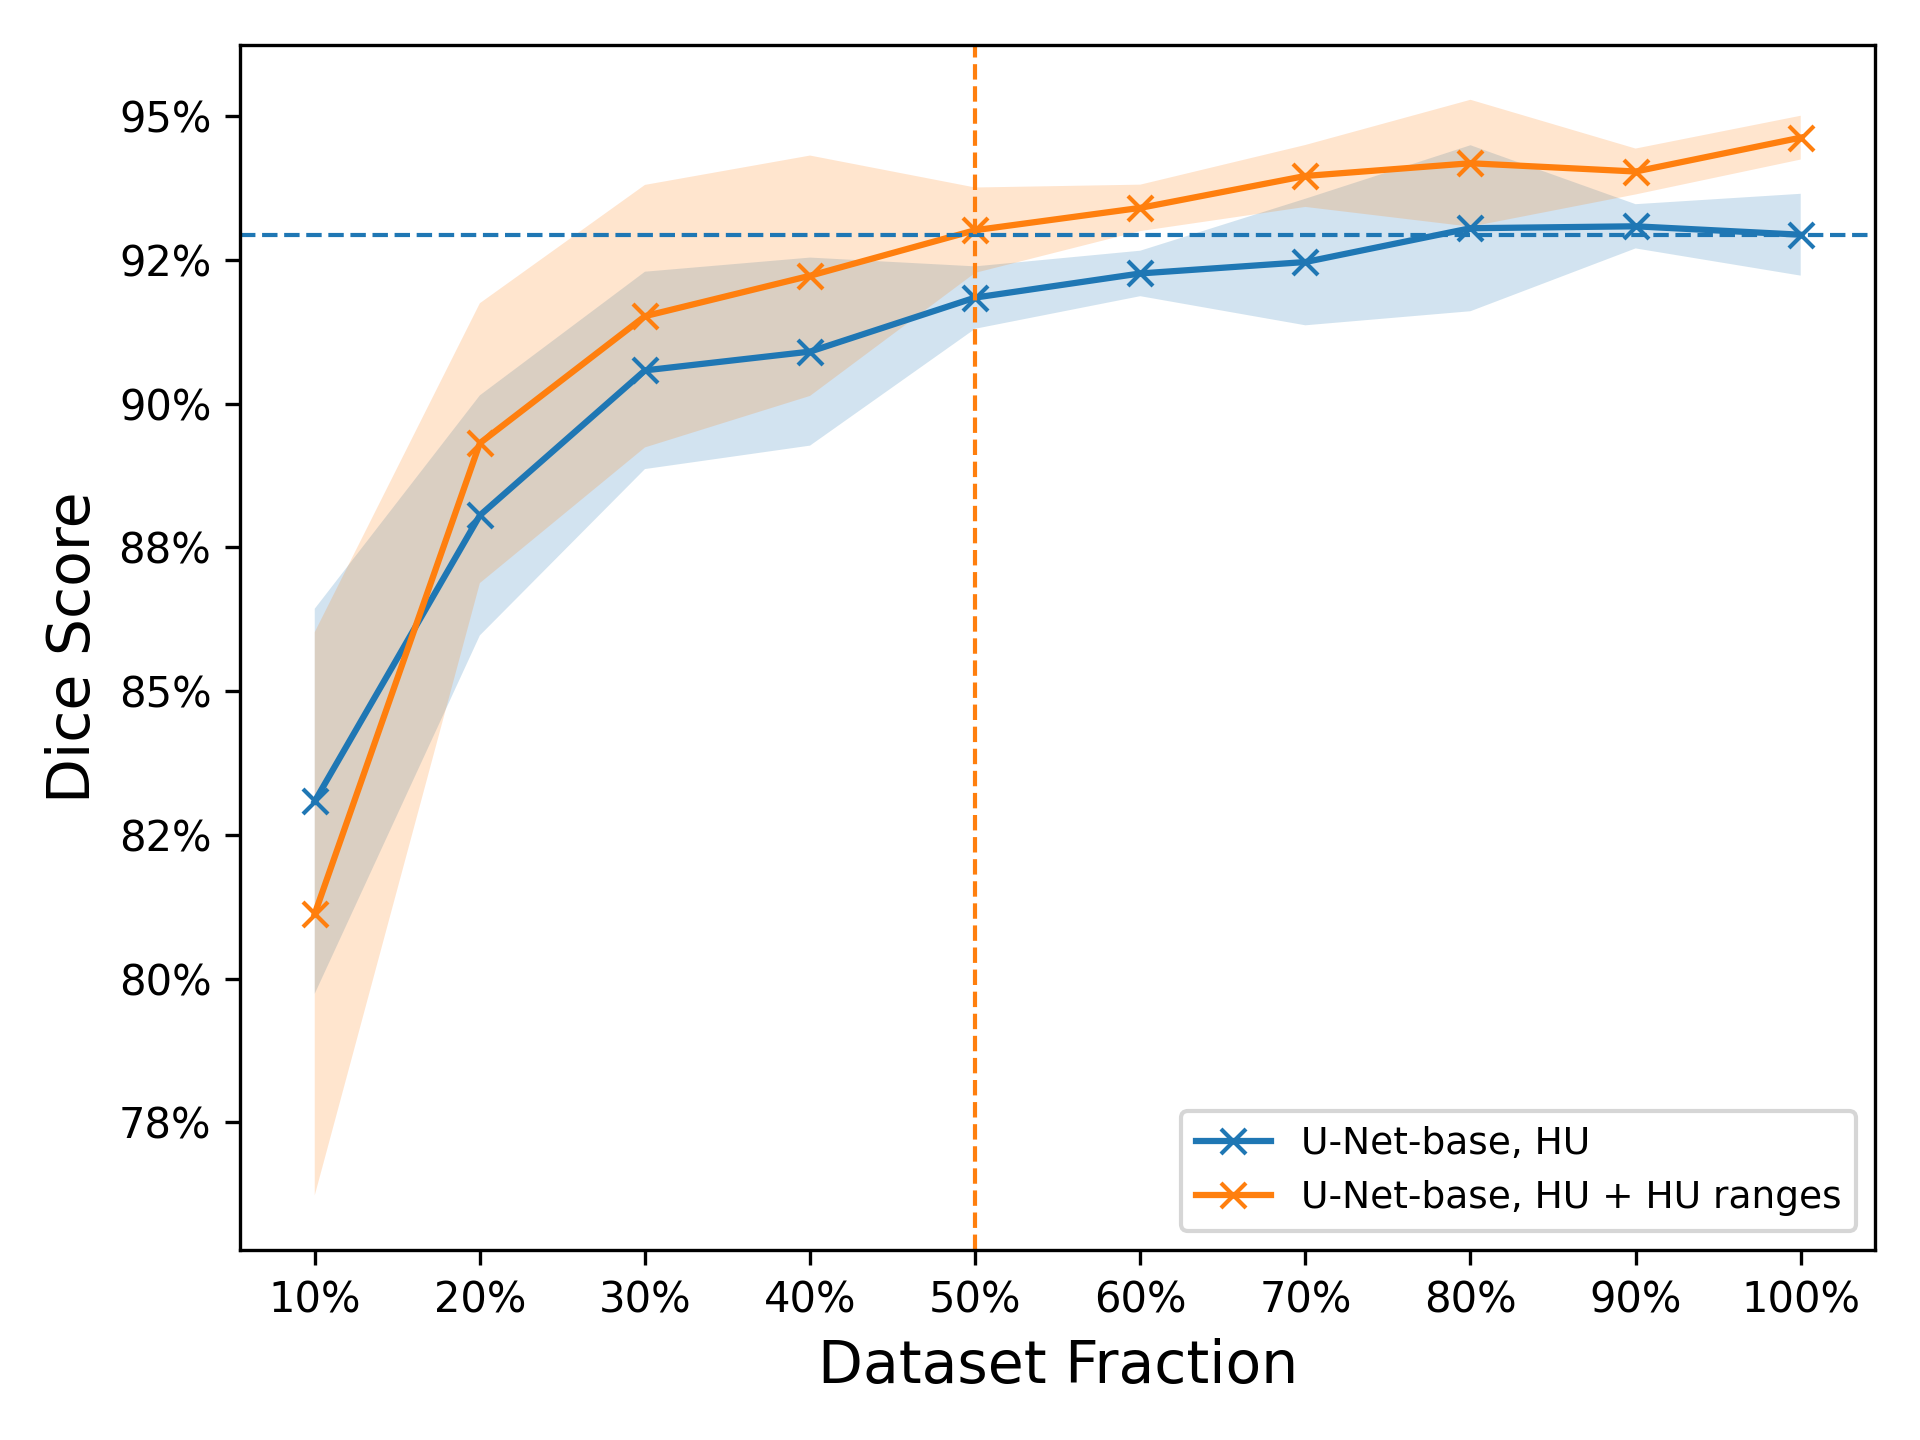
\includegraphics[width=1.0\linewidth]{figures/results/less_data_perspective_ji.png}
    \caption{Our model using HU ranges as additional features shows consistent improvement \emph{across different dataset sizes} over the baseline without them. The horizontal blue line indicates the \emph{U-Net base, HU} baseline performance using the entire dataset.
    The vertical orange line indicates that our approach surpasses this performance using \formatpercentage[round-precision=0]{0.50} of the dataset.
    % set is necessary to match the performance of the ``\emph{U-Net base, HU}'' baseline trained on all data.
    }
    \label{fig:robustness-data-size}
\end{figure}

\Cref{fig:robustness-data-size} presents the Dice score for the U-Net-base model across varying dataset fractions, comparing performance with and without the proposed HU ranges as additional features.
The results show our approach consistently improves performance by approximately \SIrange{1}{2}{\percent} across dataset fractions except for the \SI{10}{\percent} fraction.
This smallest dataset fraction only contains $4$ patients, which increases variability in cross-validation and results in wider confidence intervals.

More importantly, as highlighted in \cref{fig:robustness-data-size}, the model utilizing HU ranges surpasses the performance of the baseline when only using \SI{50}{\percent} of the training data. This finding underscores the \emph{data efficiency} of our approach, suggesting that incorporating HU ranges not only enhances segmentation accuracy but also significantly reduces the amount of labeled data needed to achieve a given performance level. Consequently, our method offers substantial practical benefits by mitigating annotation costs and improving data efficiency in training deep learning models in and for clinical practice.

\subsection{Performance improvements}

%
\begin{table*}[t]
    \caption{Experimental results. Score ranges represent the \SI{95}{\percent} confidence interval. Dice score, Precision, Recall, and F$_1$-Score are all macro averages across tissue classes.}
    \centering
    \begin{tabular}{lrrrrr}
        \toprule
        \multicolumn{1}{c}{\textbf{Model}} 
        & \multicolumn{1}{c}{\textbf{Number of parameters}} 
        % & \multicolumn{1}{c}{\textbf{Train Time Factor}} 
        & \multicolumn{1}{c}{\textbf{Dice score}} 
        & \multicolumn{1}{c}{\textbf{Precision}} 
        & \multicolumn{1}{c}{\textbf{Recall}} 
        & \multicolumn{1}{c}{\textbf{F$_1$-Score}} \\
        \midrule
        U-Net-small, HU                                   
        & \num{1943829} 
        % & \num{1.00}            
        % & \formatpercentage{0.8580}\ \ $\pm$\formatpercentage{0.0152}
        &  \hspace{15pt} \formatpercentage{0.9303}\ \ $\pm$\formatpercentage{0.002597}
        &  \hspace{5pt} \formatpercentage{0.9246}\ \ $\pm$\formatpercentage{0.01549}
        &  \hspace{5pt} \formatpercentage{0.9272}\ \ $\pm$\formatpercentage{0.009421} 
        &  \hspace{5pt} \formatpercentage{0.9252}\ \ $\pm$\formatpercentage{0.003493} \\
        U-Net-small, HU + HU ranges                       
        & \num{1944549} 
        % & \num{1.17}               
        % & \formatpercentage{0.8950}\ \ $\pm$\formatpercentage{0.0081} 
        & \formatpercentagebold{0.9467}\ \ $\pm$\formatpercentage{0.002802} 
        & \formatpercentagebold{0.9357}\ \ $\pm$\formatpercentage{0.003558} 
        & \formatpercentagebold{0.953}\ \ $\pm$\formatpercentage{0.004187} 
        & \formatpercentagebold{0.944}\ \ $\pm$\formatpercentage{0.002709} \\
        \midrule
        U-Net-base,\ \ HU                                    
        & \num{7765541}
        % & \num{1.00}  % \num{2.01}              
        % & \formatpercentage{0.8681}\ \ $\pm$\formatpercentage{0.0109} 
        & \formatpercentage{0.9359}\ \ $\pm$\formatpercentage{0.003291} 
        & \formatpercentage{0.9266}\ \ $\pm$\formatpercentage{0.004032} 
        & \formatpercentage{0.9378}\ \ $\pm$\formatpercentage{0.007159} 
        & \formatpercentage{0.9319}\ \ $\pm$\formatpercentage{0.003644} \\
        U-Net-base,\ \ HU + HU ranges                        
        & \num{7766981} 
        % & \num{1.08} % \num{2.17}   
        % & \formatpercentage{0.8980}\ \ $\pm$\formatpercentage{0.0061} 
        & \formatpercentagebold{0.9481}\ \ $\pm$\formatpercentage{0.002738} 
        & \formatpercentagebold{0.9403}\ \ $\pm$\formatpercentage{0.003056}
        & \formatpercentagebold{0.95}\ \ $\pm$\formatpercentage{0.008919}
        & \formatpercentagebold{0.9449}\ \ $\pm$\formatpercentage{0.002831}  \\
        \midrule
        U-Net-large, HU                                   
        & \num{31042629} 
        % & \num{1.00} % \num{5.82}          
        % & \formatpercentage{0.8655}\ \ $\pm$\formatpercentage{0.0087} 
        & \formatpercentage{0.9312}\ \ $\pm$\formatpercentage{0.005912} 
        & \formatpercentage{0.9263}\ \ $\pm$\formatpercentage{0.01057} 
        & \formatpercentage{0.9273}\ \ $\pm$\formatpercentage{0.02222}
        & \formatpercentage{0.9261}\ \ $\pm$\formatpercentage{0.007489} \\
        U-Net-large, HU + HU ranges                       
        & \num{31045509}          
        % & \num{1.02} % \num{5.93}               
        % & \formatpercentage{0.8913}\ \ $\pm$\formatpercentage{0.0039} 
        & \formatpercentagebold{0.9455}\ \ $\pm$\formatpercentage{0.001213} 
        & \formatpercentagebold{0.9316}\ \ $\pm$\formatpercentage{0.003021} 
        & \formatpercentagebold{0.953}\ \ $\pm$\formatpercentage{0.006178} 
        & \formatpercentagebold{0.9419}\ \ $\pm$\formatpercentage{0.001499}  \\
        \bottomrule
    \end{tabular}
    \label{tab:results} \label{tbl:results}
\end{table*}

\Cref{tbl:results} summarizes the experimental results, comparing the performance of U-Net models of varying sizes with and without our proposed approach of incorporating HU ranges as additional features to learn from.
Across all model sizes, the inclusion of HU ranges consistently improves segmentation performance across multiple metrics, with the Dice score improving by approximately \SIrange{1}{2}{\percent}, reducing the remaining error by \SI{20}{\percent}. 
The improvements hold consistently across different U-Net model sizes and dataset fractions, demonstrating the applicability across diverse training settings.

Our baseline results without our proposed additional inputs align with previously reported findings on similar datasets.
For example, \cite{ha_development_2021} achieve a Dice score of \formatpercentage[round-precision=0]{0.97} using their internal dataset of $1496$ CT scans of the L3 vertebra from $922$ patients, segmenting the tissue types SM, SAT, and VAT.
Our \emph{U-Net-base, HU} model achieves a comparable Dice score of \formatpercentage[round-precision=0]{0.9492} on the same tissue types (i.e., when ignoring IMAT) despite using a smaller dataset of only $176$ CT scans from $44$ patients for training and evaluation.

By expanding the number of input channels with engineered masks, the first convolution has few additional parameters, leading to increased computational demand and memory needs.
Empirically, we found that the training time was at most $1.17\times$ higher than the network without the HU ranges.
This efficiency makes our approach both computationally feasible and practically advantageous.  

\subsection{Performance per tissue type}

\begin{figure}[t]
\centering
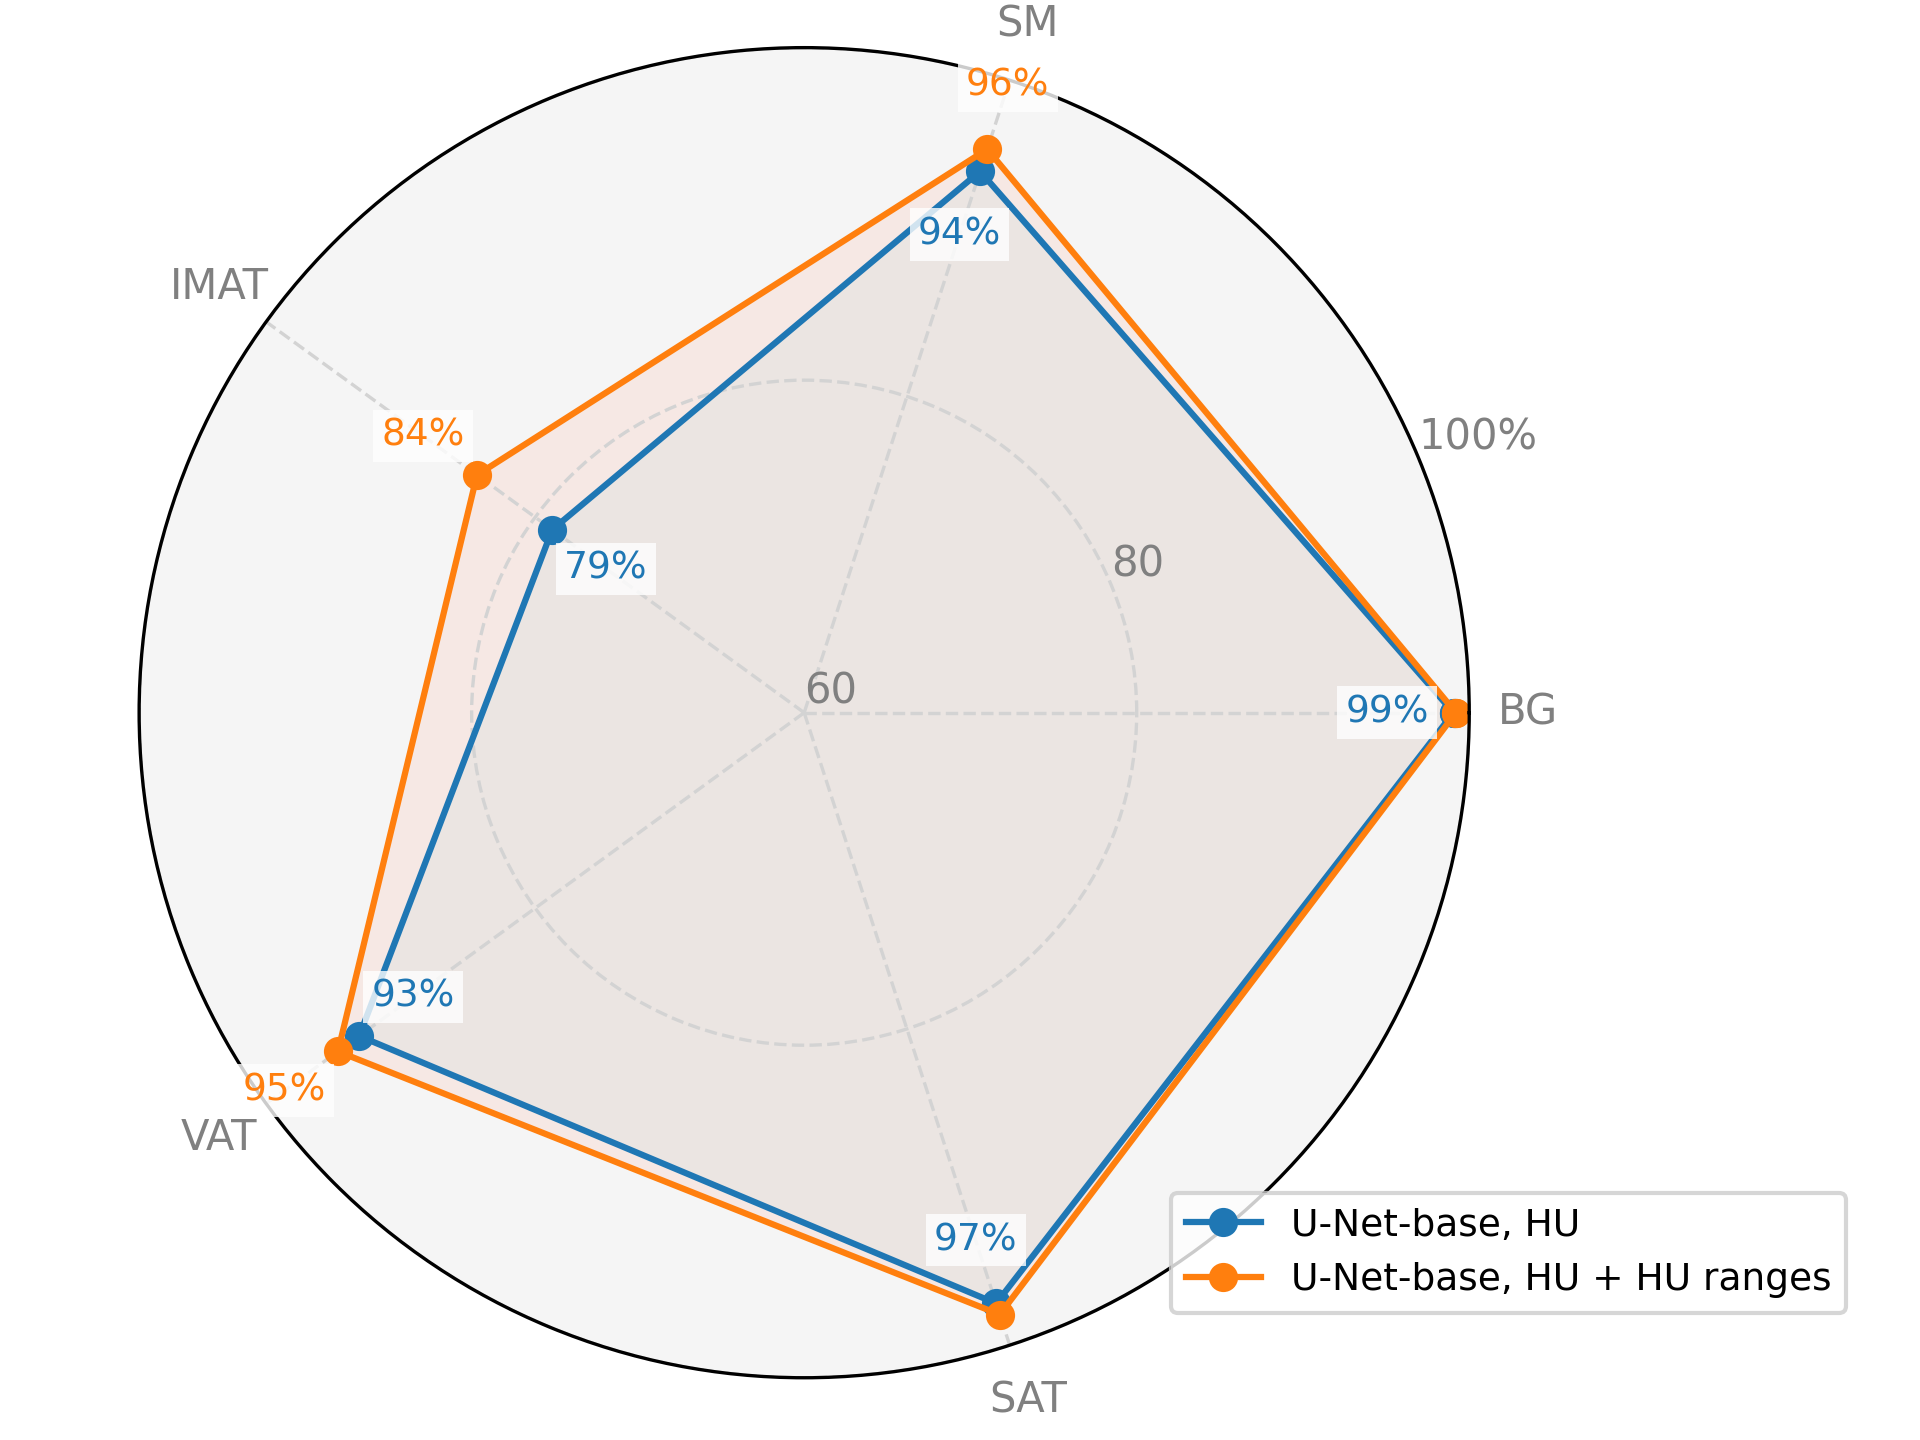
\includegraphics[width=1.0\linewidth]{figures/results/base_tissue_types.png}
\caption{Dice score \emph{per tissue type} and background (BG). Giving the model a physiology-informed inductive bias via HU ranges-based masks keeps (BG, SAT) or improves performance, with IMAT improvements being of high clinical value.}
\label{fig:tissue-types}
\end{figure}

\Cref{fig:tissue-types} shows the dice score per tissue type for the U-Net-base model, comparing performance with and without the inclusion of HU ranges.
While the segmentation performance remains nearly identical for background and SAT, a modest improvement is observed for SM and VAT.
However, a substantial performance increase of approximately \SI{5}{\percent} is achieved for IMAT.


IMAT is recognized as an important biomarker for various medical diagnoses \cite{lim_inter-muscular_2019, suka_aryana_important_2023}, yet it remains challenging to segment it accurately \cite{hemke_deep_2020, paris_automated_2020} because its regions are smaller and more spread out than other tissues.
Thus, the incorporation of HU ranges not only enhances overall segmentation performance but also significantly improves the detection of IMAT, a clinically relevant yet difficult-to-identify tissue type.


\section{Ablation Studies}

\subsection{Removing raw HU values}

To evaluate the sufficiency of the derived features $\bm{X}_c$ alone, we conduct experiments excluding the original HU values $\bm{X}_0$ (the original CT image) from the input. This modification reduces the available input information, as the binary masks are \emph{derived from} the HU values but are \emph{not invertible}.
However, as shown in \cref{tbl:results-hut}, the performance remains high across all model sizes, even surpassing the results obtained with raw HU values alone (\cref{tbl:results}).
This confirms that the inductive bias introduced by our ``feature engineering'' provides a more effective representation of the information needed for semantic segmentation of CT images with respect to BCA.

\begin{table}[t]
    \caption{Segmentation performance when trained using only binary masks (excluding raw HU values from the CT images).}
     \begin{center}
    \begin{tabular}{lrr}
        \toprule
        \multicolumn{1}{c}{\textbf{Model}} 
        & \multicolumn{1}{c}{\textbf{Dice score}} 
        & \multicolumn{1}{c}{\textbf{F$_1$-Score}} \\
        \midrule
        U-Net-small, (only) HU ranges                      
        % & \formatpercentage{0.8906}\ \ $\pm$\formatpercentage{0.0036} 
        & \formatpercentage{0.9424}\ \ $\pm$\formatpercentage{0.002643} 
        & \formatpercentage{0.9383}\ \ $\pm$\formatpercentage{0.003656}  \\
        \midrule
        U-Net-base,\ \ (only) HU ranges
        % & \formatpercentage{0.8933}\ \ $\pm$\formatpercentage{0.0021} 
        & \formatpercentage{0.9439}\ \ $\pm$\formatpercentage{0.002513} 
        & \formatpercentage{0.94}\ \ $\pm$\formatpercentage{0.002301} \\
        \midrule
        U-Net-large, (only) HU ranges                       
        % & \formatpercentage{0.8854}\ \ $\pm$\formatpercentage{0.0041}
        & \formatpercentage{0.9403}\ \ $\pm$\formatpercentage{0.003839}  
        & \formatpercentage{0.9356}\ \ $\pm$\formatpercentage{0.003553} \\
        \bottomrule
    \end{tabular}
    \label{tab:results-no-hu-values} \label{tbl:results-hut}
     \end{center}
\end{table}

\subsection{Removing individual binary masks during inference} \label{sec:remove-masks}

To further evaluate the contribution of individual binary masks, we measure the performance drop when artificially removing a single binary mask \emph{during inference} by setting all locations to zero. 
\Cref{tbl:results-removed-mask} presents the results using the final checkpoint of our \emph{U-Net-base, HU + HU ranges} model.

The middle column shows the drop in performance for a specific tissue type if its binary mask is removed.
The segmentation performance for SM and VAT drops substantially to \SI{0}{\percent} when we remove their corresponding binary mask at inference, suggesting that the trained model relies heavily on the binary masks to segment these tissue types.
Since IMAT and SAT share identical thresholds (\Cref{tab:hu_values}), we remove their (identical) binary masks together.
Removing those masks results in a notable decrease in segmentation performance, particularly for IMAT, where the score drops by over \SI{70}{\percent}.
Overall, the results in the middle column suggest that the model utilizes a tissue's binary mask to segment the specific tissue type.

The right column shows the drop in performance for the \emph{remaining} tissue classes (all tissue classes whose masks we did not remove).
Notably, this score is also affected, dropping \SI{24}{\percent} if we remove the SM binary mask and around \SIrange{8}{9}{\percent} if removing other masks.
While we suspect that the binary masks help the model to better detect other tissue types as well,
this overall performance drop on other tissue types could also be due to having unrealistic input, as the binary masks don't match the CT input image, and thus are out of distribution.
% introduced by our feature engineering is not only leveraged by the model but also contributes strongly to the model's final performance.

\begin{table}[h]
    \caption{
    Effect of removing individual binary masks during inference. Numbers (left $\rightarrow$ right) show the Dice score drop from the unchanged binary mask (left) to the removed binary mask (right).
    The first column shows which tissue's binary mask we remove.
    The second column shows the Dice score drop for the tissue classes whose mask we remove.
    The third column shows the Dice score drop for the \emph{remaining} tissue classes (all tissue classes whose masks we did not remove).
    Last row: As IMAT and SAT share the same HU range, they are removed together, with the first tissue Dice score for IMAT and the second for SAT.
    }
    \begin{center}
    \begin{tabular}{lrr}
        \toprule
        \multicolumn{1}{c}{\textbf{Removed mask}} 
        & \multicolumn{1}{c}{\textbf{Tissue Dice score}}
        & \multicolumn{1}{c}{\textbf{Other Dice score}} \\
        \midrule
        SM
        & \formatpercentage{0.9508} $\rightarrow$\ \ \ \SI{0.0}{\percent}     
        & \formatpercentage{0.9338} $\rightarrow$ \formatpercentage{0.6930}  \\   
        \midrule
        VAT
        & \formatpercentage{0.9409} $\rightarrow$\ \ \ \SI{0.0}{\percent}
        & \formatpercentage{0.9344} $\rightarrow$ \formatpercentage{0.8476} \\

        \midrule
        \multirow{2}{*}{\shortstack[l]{IMAT and \\ SAT}}
        %\midrule
        %IMAT (+ SAT)
        & \formatpercentage{0.8322} $\rightarrow$ \formatpercentage{0.1064}
        & \multirow{2}{*}{\formatpercentage{0.9484} $\rightarrow$ \formatpercentage{0.8651}} \\
        & \formatpercentage{0.9800} $\rightarrow$ \formatpercentage{0.6846} & \\
        \bottomrule
    \end{tabular}
    \label{tbl:results-removed-mask}
    \end{center}
\end{table}


\section{Discussion and Conclusions}
We introduced a new method for semantic segmentation of CT images for BCA by adding binary masks derived from medical textbook knowledge of HU ranges per tissue class to each input image as additional channels. Considering this physiology-informed prior knowledge as an inductive bias, our model achieves enhanced segmentation performance with drastically reduced labeled training data requirements:
We show a consistent improvement across dataset and model sizes and, in our case, that our model surpasses the performance of the baseline model using only \SI{50}{\percent} of the data.

Compared to a related method that uses multiple HU windows \cite{kloenne_domain-specific_2020}, our method achieves superior results, especially in the data-limited setting (see \cref{sec:hu-windowing} for details).
%and complementing conventional data efficiency techniques such as data augmentation.

The standardized nature of HU ranges ensures broad applicability of our approach across diverse clinical settings, facilitating CT segmentation in resource-limited environments. This has direct implications for clinical practice in tasks like BCA, aiding in identifying conditions such as sarcopenia and obesity.

Despite these advantages, HU-based binary masks provide a coarse tissue approximation and may introduce ambiguities where HU ranges overlap, such as between muscle and different types of adipose tissue. Addressing these limitations in future work with adaptive thresholding or probabilistic priors could refine performance. Additionally, incorporating additional anatomical constraints or shape priors may further enhance segmentation robustness.
Furthermore, the proposed approach should be evaluated on different datasets and tasks to demonstrate its broad generalizability.

In conclusion, our results highlight the efficacy of leveraging physiology-informed inductive bias in medical image segmentation, demonstrating a broadly applicable approach that optimizes data efficiency and facilitates clinical applicability.


\bibliography{references_clean}
\bibliographystyle{IEEEtran}

\vfill

\appendix

\section{Comparing to HU Windowing}\label{sec:hu-windowing}

HU windowing is an alternative pre-processing technique proposed by \cite{kloenne_domain-specific_2020}, which, like our approach, incorporates the HU ranges as an inductive bias.
Instead of utilizing binary masks, HU windowing creates multiple HU windows by clipping the HU values to each HU range and normalizing the values.
For a given tissue class $c$, let $L_{c}$ and $U_{c}$ denote the lower and upper bounds of the HU range, respectively. The transformed input representation is then defined as:
%
\begin{equation}
X_{c}(i,j) = \begin{cases}
    \frac{L_c}{|U_c - L_c|}, & \text{if } X_{0}(i,j) < L_{c},\\
    \frac{U_c}{|U_c - L_c|}, & \text{if } X_{0}(i,j) > U_{c},\\
    \frac{X_{0}(i,j)}{|U_c - L_c|}, & \text{otherwise}.
\end{cases}
\label{eq:pixel_clipping}
\end{equation}
%
% While HU windowing has been reported to improve segmentation performance, it remains relatively underexplored in practice. 
% To assess its efficacy compared to our proposed binary mask encoding, we conducted experiments using both approaches.
The results using HU windowing in \cref{tbl:hu-windowing} indicate that while our results are slightly superior, both inductive bias strategies yield comparable performance across different model sizes.
However, binary masks have a stronger inductive bias as HU values are \emph{reduced} to binary values, leading to fewer possible inputs.
Consequently, models trained with binary masks should learn simpler yet more robust patterns independent of the specific HU values.
\Cref{fig:hu-window-data} indicates that our approach works better in \emph{data-limited} circumstances, but further investigation is required to determine whether specific segmentation tasks or dataset characteristics favor one encoding method over the other.

\begin{table}[h]
    \caption{Results of HU windowing on our dataset.}
    \begin{center}
    \begin{tabular}{lr}
        \toprule
        \multicolumn{1}{c}{\textbf{Model}} 
        & \multicolumn{1}{c}{\textbf{Dice score}} \\
        \midrule
        U-Net-small, HU windows                    
        % & \formatpercentage{0.8804}\ \ $\pm$\formatpercentage{0.0048} \\               
        & \formatpercentage{0.9367}\ \ $\pm$\formatpercentage{0.004573} \\               
        \midrule
        U-Net-base,\ \ HU windows
        % & \formatpercentage{0.8840}\ \ $\pm$\formatpercentage{0.0066} \\               
        & \formatpercentage{0.9409}\ \ $\pm$\formatpercentage{0.003887} \\
        \midrule
        U-Net-large, HU windows                       
        % & \formatpercentage{0.8872}\ \ $\pm$\formatpercentage{0.0033} \\
        & \formatpercentage{0.9402}\ \ $\pm$\formatpercentage{0.002434} \\
        \bottomrule
    \end{tabular}
    \label{tbl:hu-windowing}
    \end{center}
\end{table}
\vspace{-2em}
\begin{figure}[h]
    \centering
    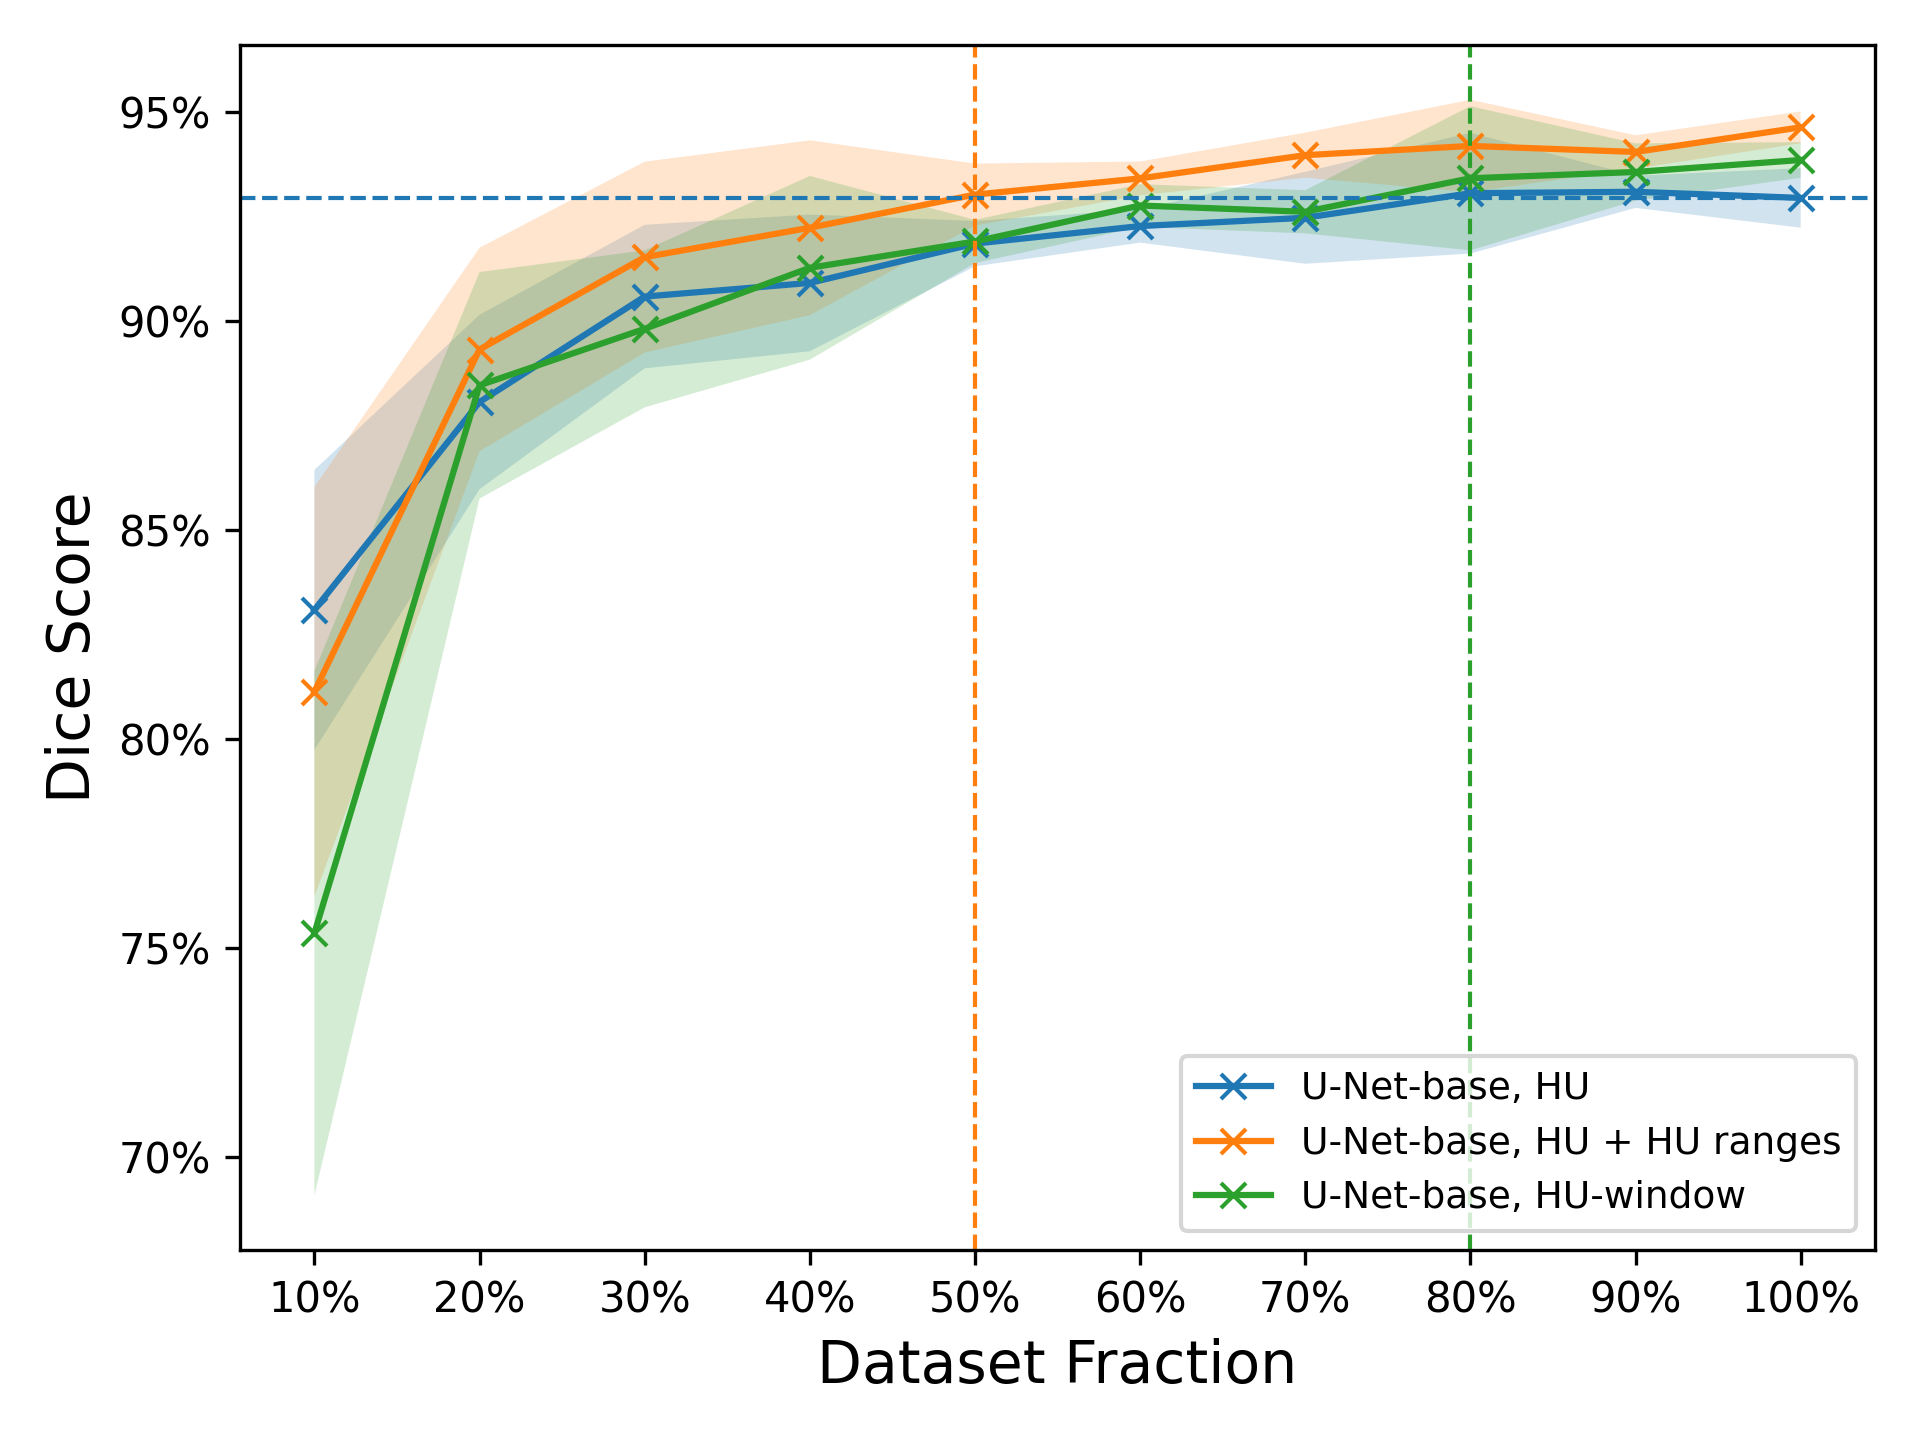
\includegraphics[width=1.0\linewidth]{figures/results/hu-window-data.png}
    \caption{\Cref{fig:robustness-data-size} with HU windowing experiments added. The vertical green line indicates that HU windowing surpasses the baseline performance with \SI{80}{\percent} of the dataset.}
    \label{fig:hu-window-data}
\end{figure}

\end{document}
